\documentclass{beamer}
\usepackage[utf8]{inputenc}
\usepackage[T1]{fontenc}
\usepackage[polish]{babel}
\usepackage{graphicx}
\usepackage{times}
\usepackage{color}
\usepackage{colortbl}
\usetheme{AGH}

\title[Biometryczny System Kontroli Dostępu]{Biometryczny System Kontroli Dostępu}

\author[T. Drzewiecki, J. Gajda]{Tomasz Drzewiecki, Joanna Gajda}

\date[2012]{17.01.2012}

\institute[AGH-UST]
{Wydział Elektrotechniki, Automatyki, Informatyki i Elektroniki\\ 
Katedra Automatyki
}

\setbeamertemplate{itemize item}{$\maltese$}

\begin{document}

{
%\usebackgroundtemplate{
\includegraphics[width=\paperwidth]{titlepage}} % wersja angielska
\usebackgroundtemplate{
\includegraphics[width=\paperwidth]{titlepagepl}} % wersja polska
 \begin{frame}
   \titlepage
 \end{frame}
}

%---------------------------------------------------------------------------

\begin{frame}
\frametitle{Tematyka projektu}

\begin{block}{Cel projektu}
Celem naszego projektu było stworzenie/rozbudowa systemu do identyfikacji osób na podstawie tęczówki oka.
\end{block}

\begin{figure}
\begin{center}
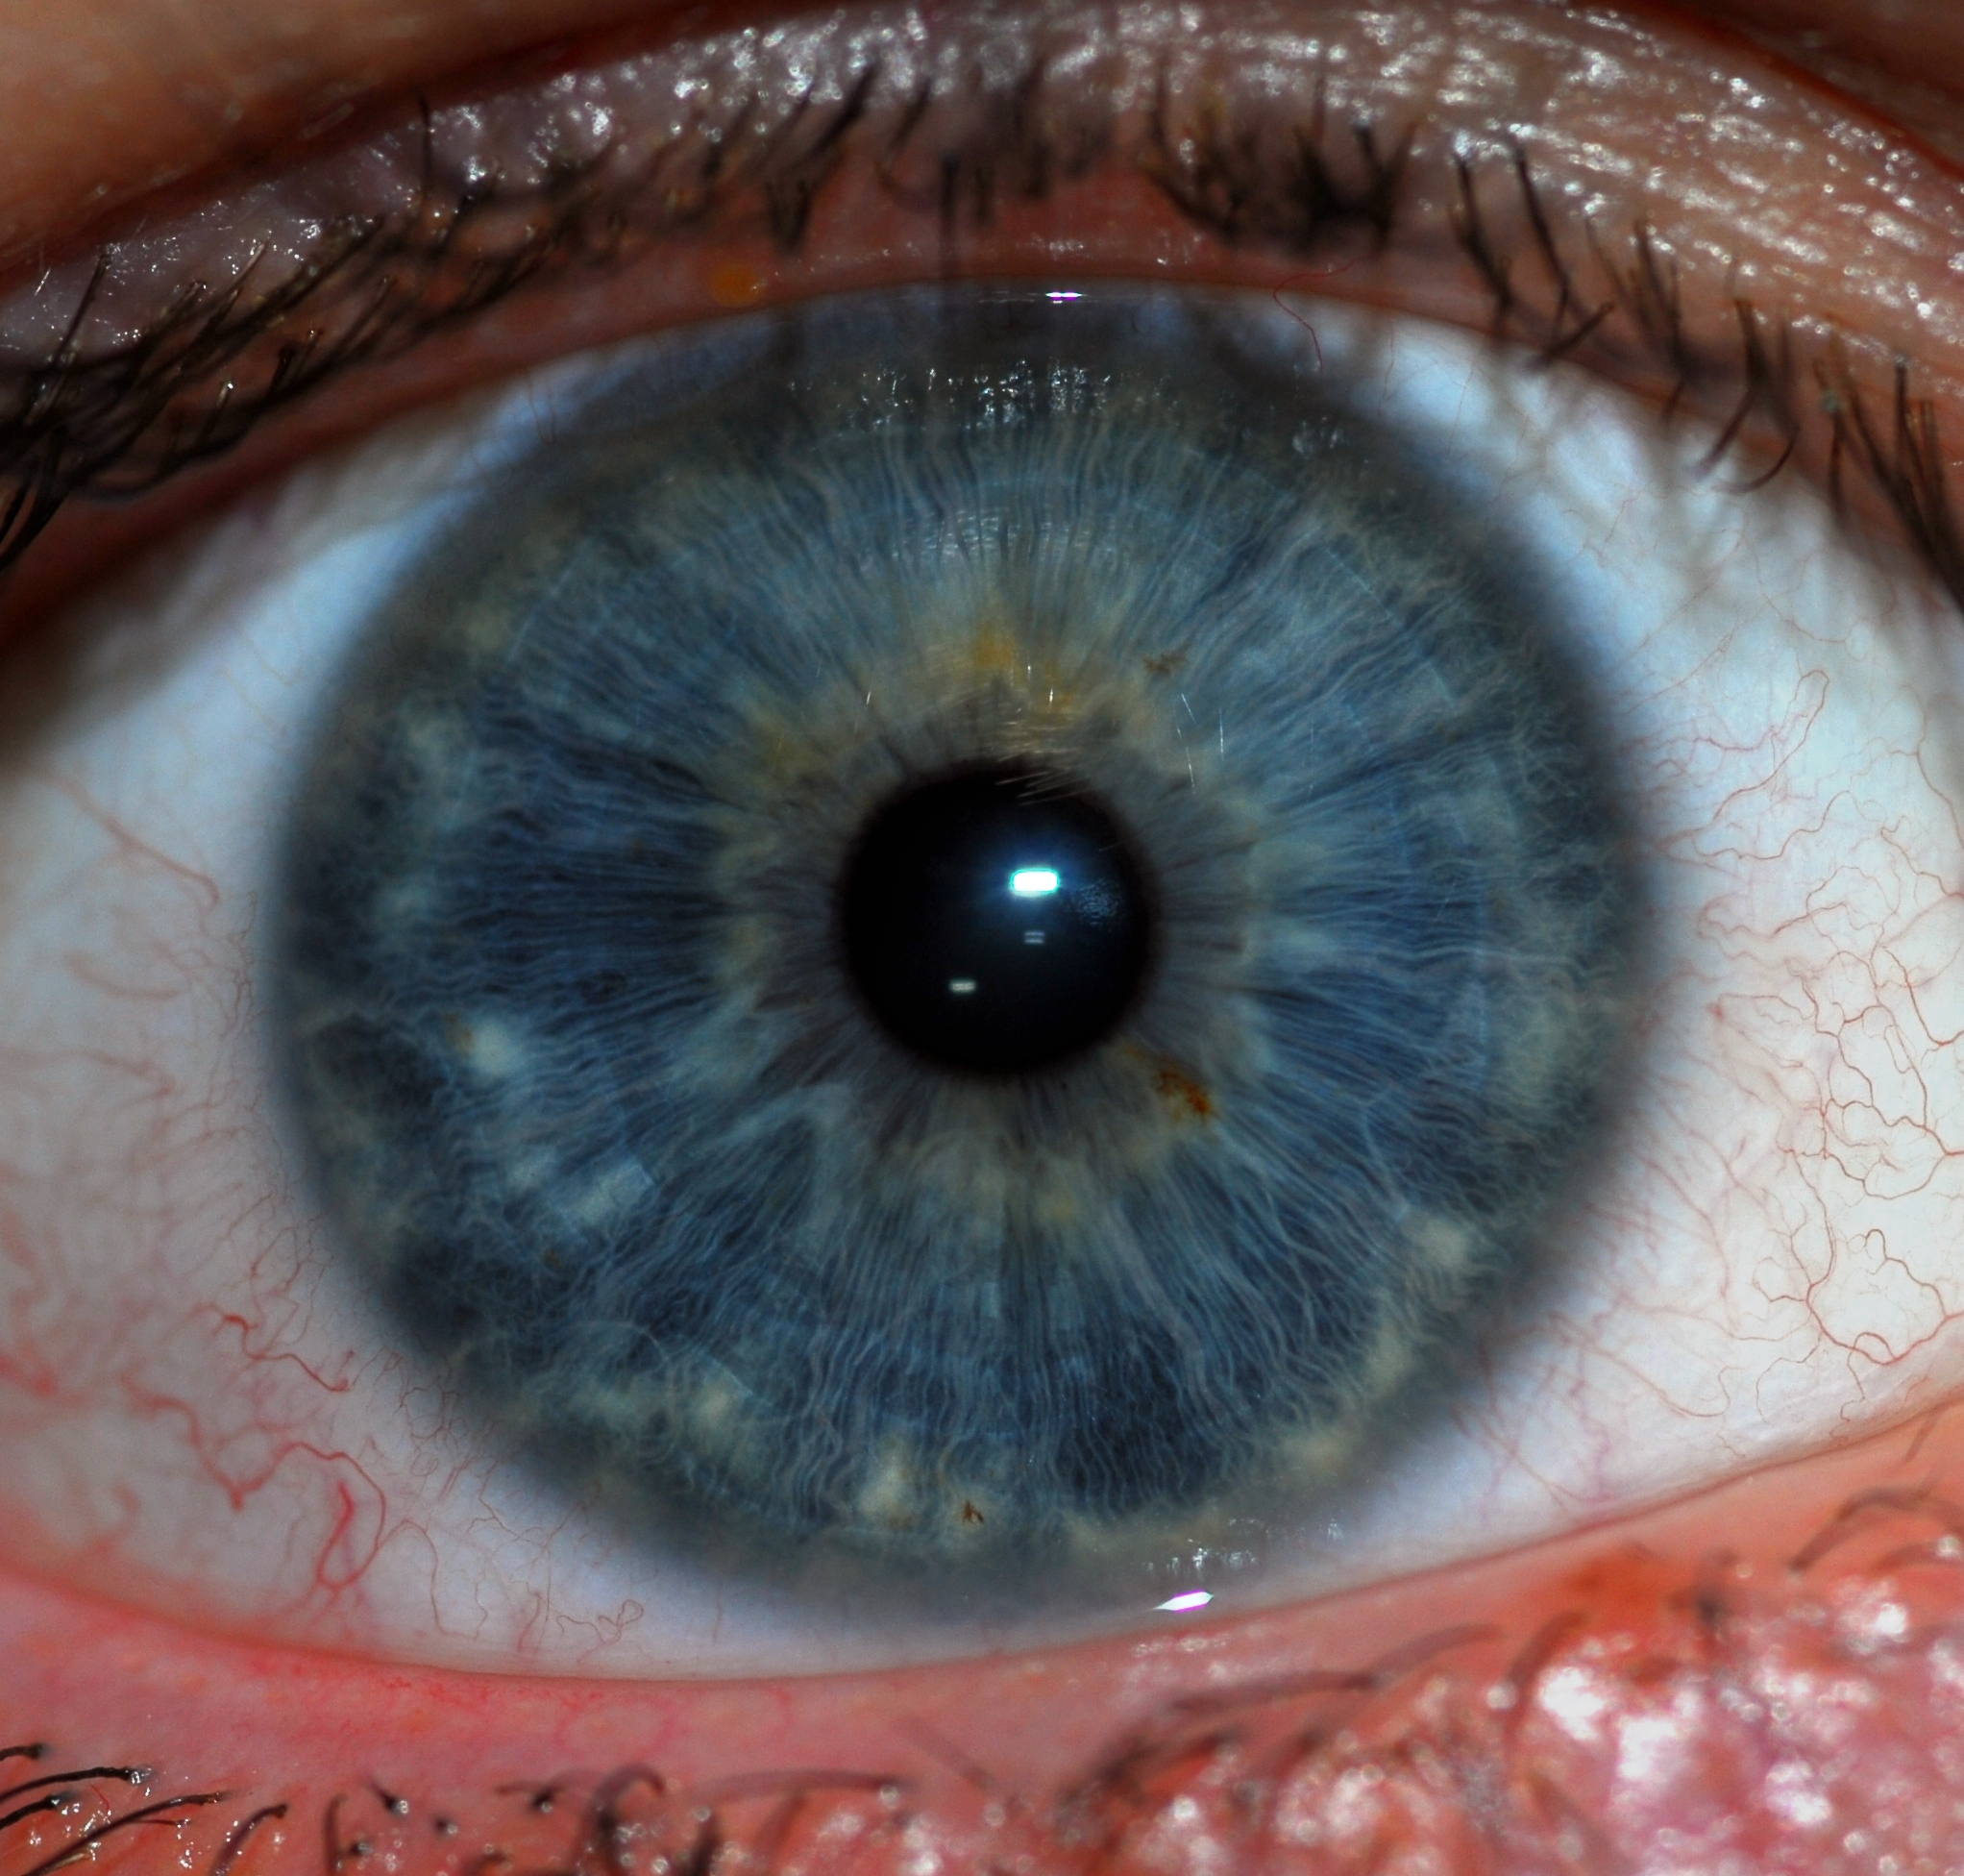
\includegraphics[scale=0.04]{teczowka.jpg}
\caption{Tęczówka człowieka}
\end{center}
\end{figure}

\end{frame}

%---------------------------------------------------------------------------

\begin{frame}
\frametitle{Podział systemu}
\begin{columns}[t]
\column{0.3\textwidth}
\begin{block}{Część sprzętowa}
Moduł odpowiedzialny za pobranie obrazu tęczówki od badanych osób. Najważniejszym elementem jest kamera oraz zapewnienie odpowiednich warunków.
\end{block}
\column{0.3\textwidth}
\begin{block}{Cześć biometryczna}
Część odpowiedzialna na zamianę obrazu tęczówki na jej kod oraz późniejsze porównywanie utworzonych kodów.
\end{block}
\column{0.3\textwidth}
\begin{block}{Część bazodanowa}
Część odpowiedzialna za przechowywanie danych osób wprowadzanych do systemu.
\end{block}
\end{columns} 

\end{frame}

%---------------------------------------------------------------------------

\begin{frame}
\frametitle{Konstrukcja stanowiska}
Stanowisko do pobierania obrazów musi spełniać odpowiednie wymagania. Główne założenia oraz ich realizacja:
\begin{itemize}
\item Likwidacja odblasków pochodzących z oświetlenia (naturalnego oraz sztucznego) - zastosowanie kartonowego pudła,
\item Odpowiednia jasność obrazu - zastosowanie oświetlacza IR,
\item Wysoka jakość obrazu - zastosowanie odpowiedniej kamery,
\item Odpowiednia wielkość tęczówki na obrazie - zastosowanie odpowiedniego obiektywu.
\end{itemize}
\end{frame}
%---------------------------------------------------------------------------

\begin{frame}
\frametitle{Stworzone stanowisko}
\begin{columns}
	\column{0.5\textwidth}
		\begin{figure}
		\begin{center}
		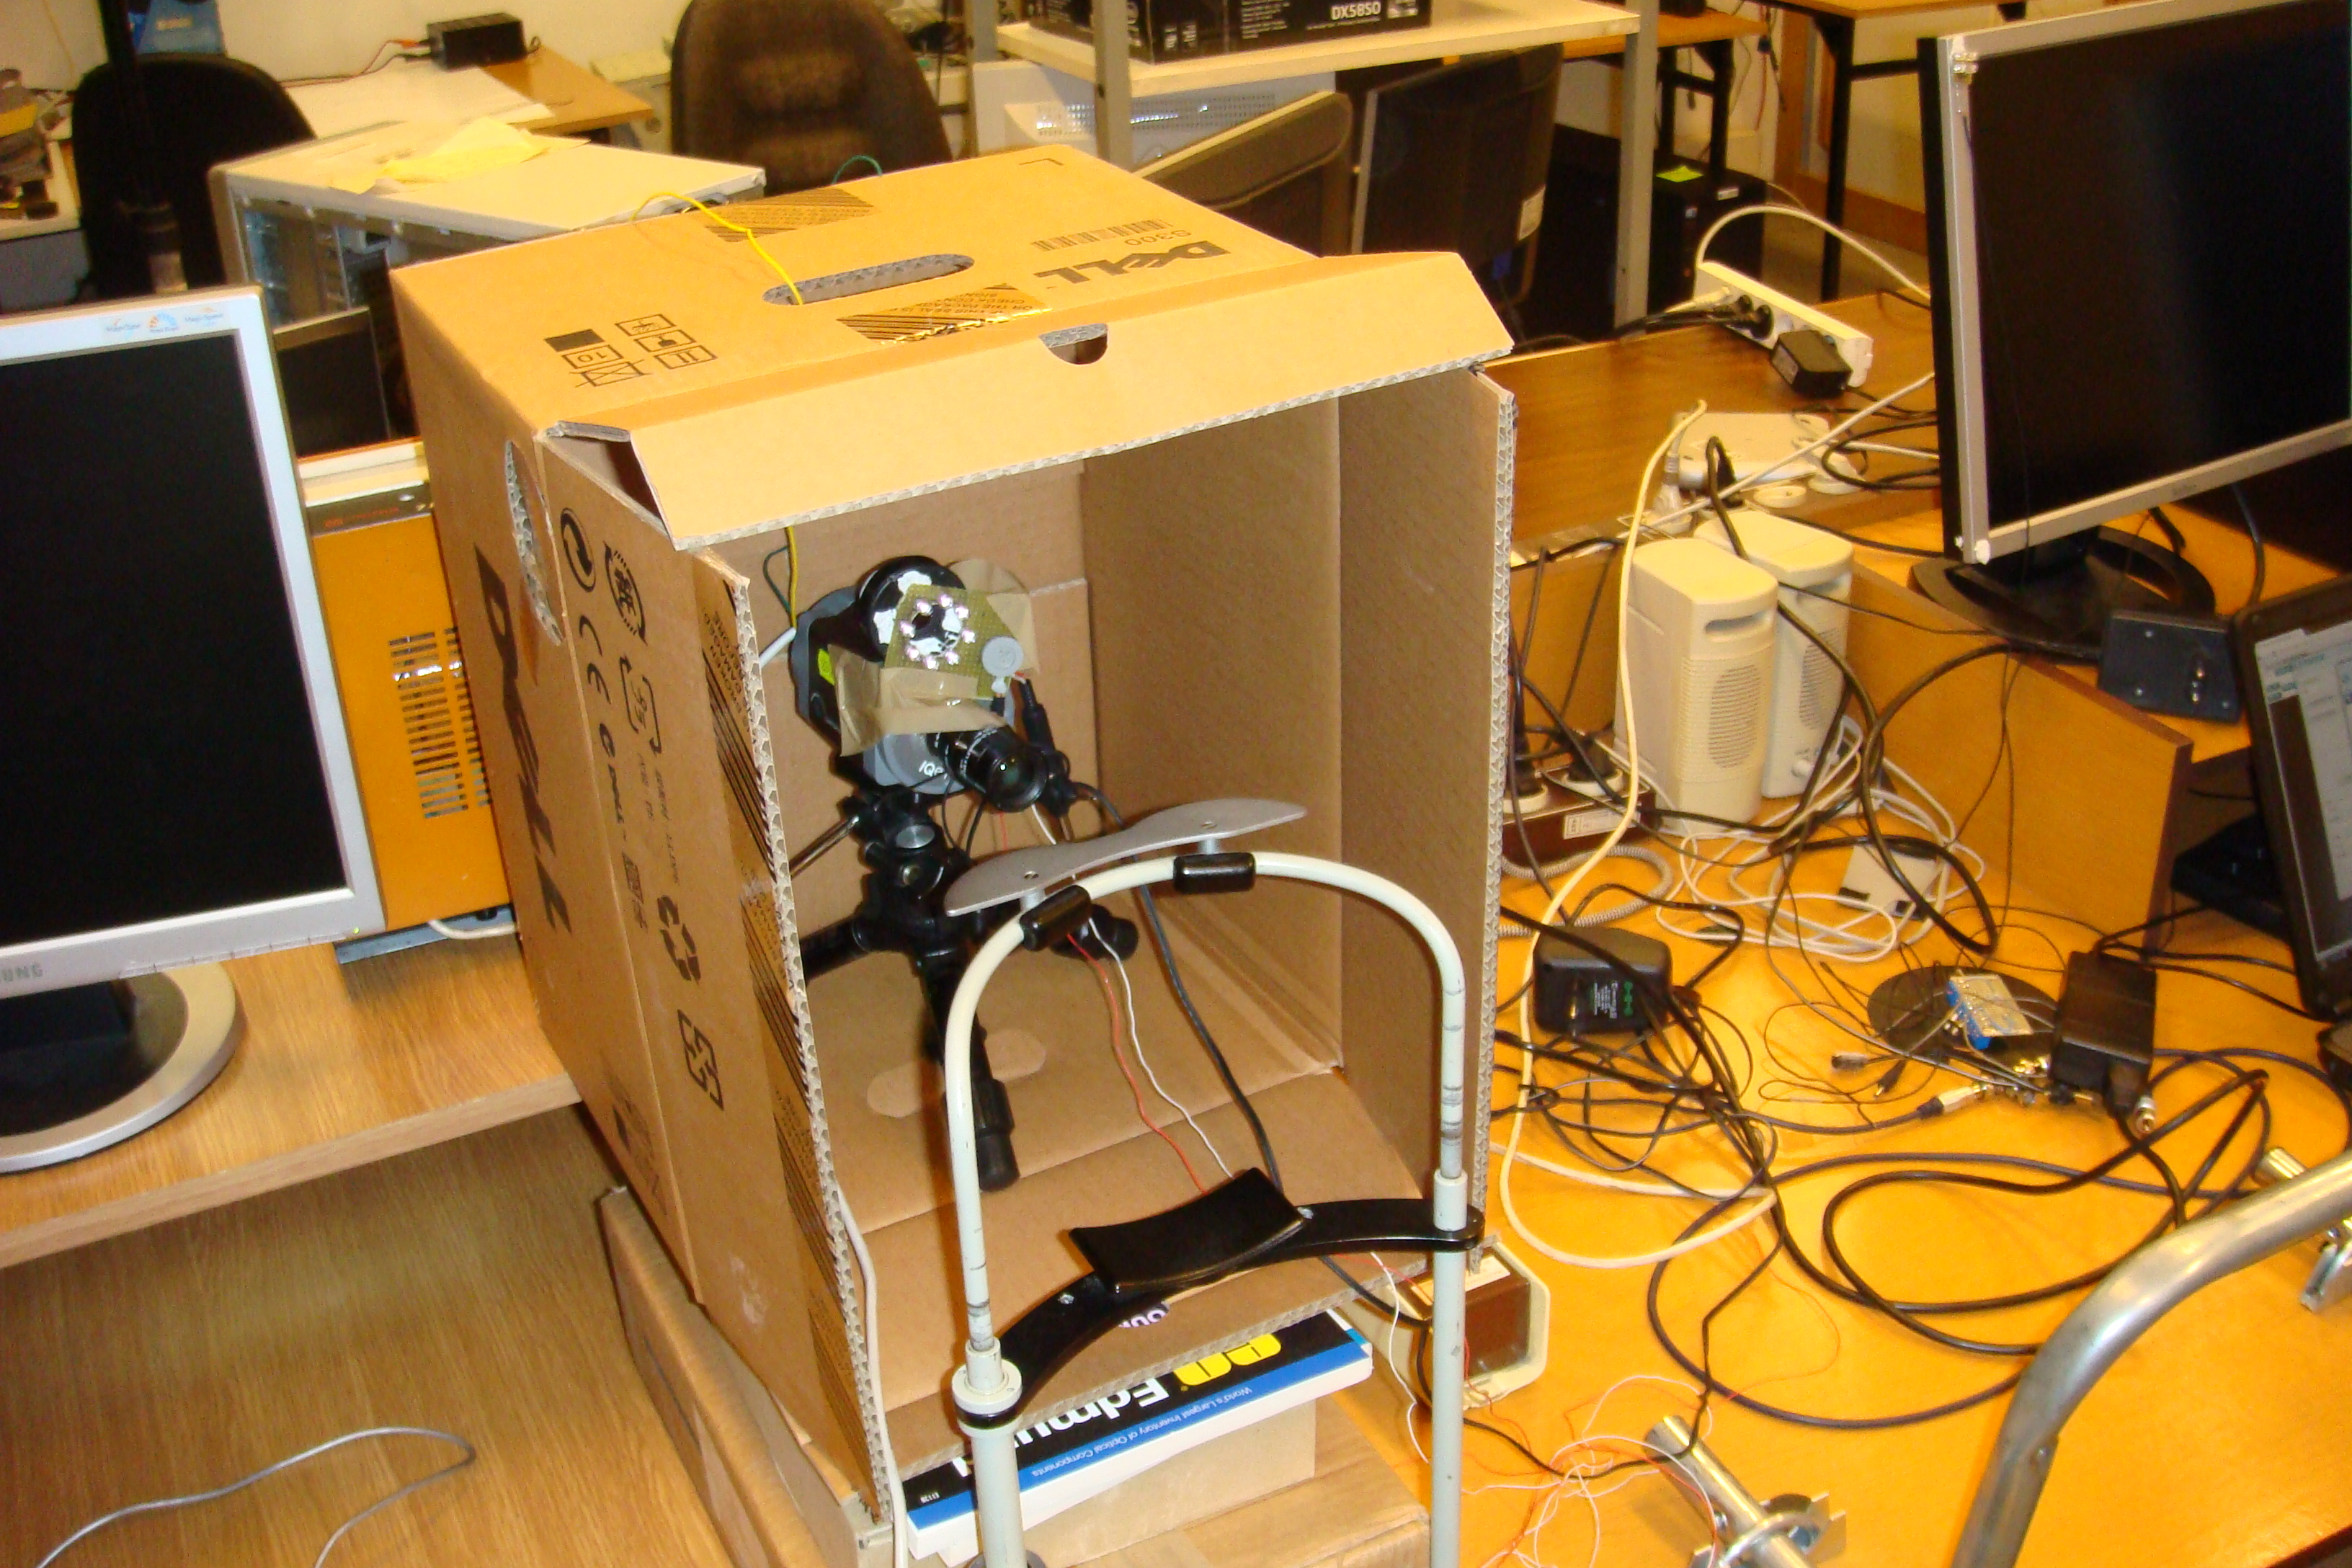
\includegraphics[scale=0.05]{stanowisko1.jpg}
%		\caption{Obraz przed czyszczeniem brzegów}
		\end{center}
		\end{figure}
	\column{0.5\textwidth}
		\begin{figure}
		\begin{center}
		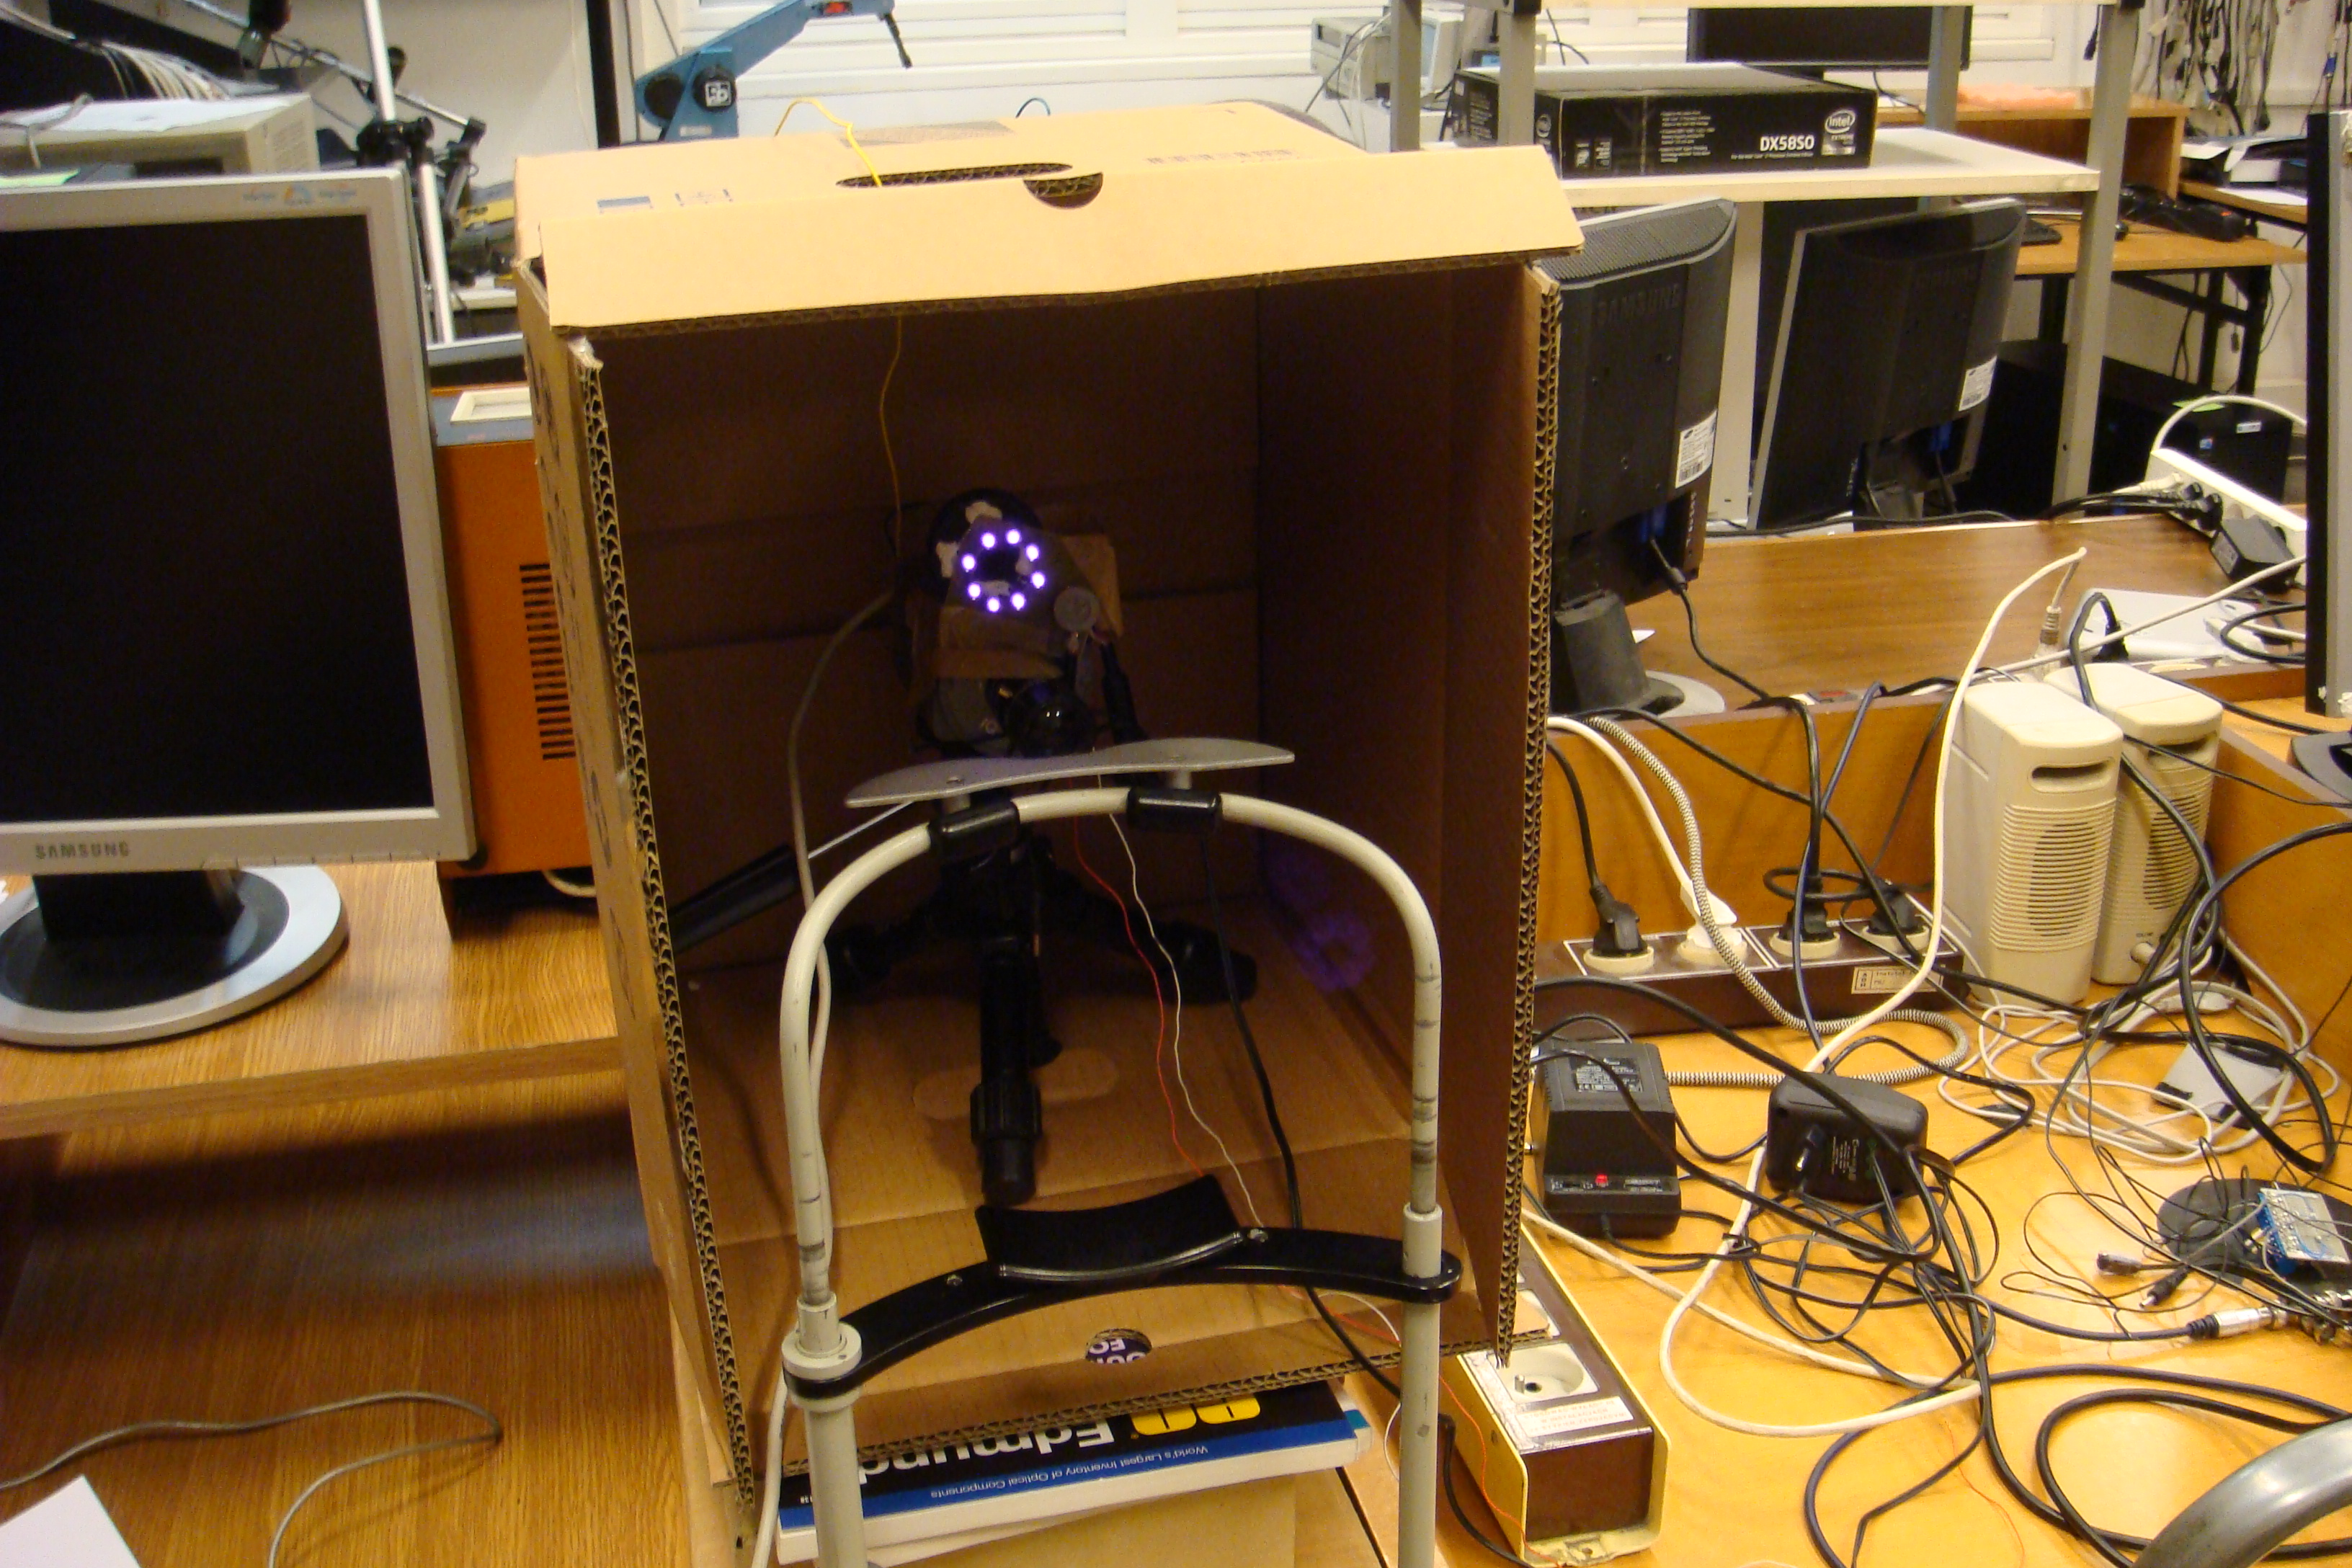
\includegraphics[scale=0.05]{stanowisko2.jpg}
%		\caption{Obraz po czyszczenu brzegów}
		\end{center}
		\end{figure}
\end{columns}\end{frame}

%---------------------------------------------------------------------------

\begin{frame}
\frametitle{Algorytm do tworzenia kodu tęczówki}
\begin{figure}
\begin{center}
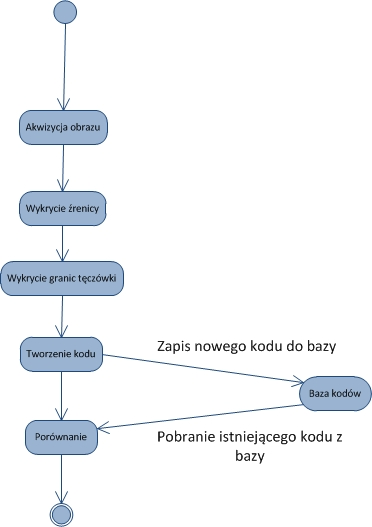
\includegraphics[scale=0.45]{schemat.jpg}
\end{center}
\end{figure}
\end{frame}

%---------------------------------------------------------------------------

\begin{frame}
\frametitle{Wykrycie źrenicy}
Celem tej części algorytmu jest opisanie źrenicy przy pomocy okręgu. Pierwszym etapem wyszukiwania źrenicy jest znalezienie odblasku widocznego na źrenicy pochodzącego od oświetlacza IR. Do dalszych przekształceń wybierany jest odpowiedni fragment obrazu zaznaczony na rysunku.
\begin{figure}
\begin{center}
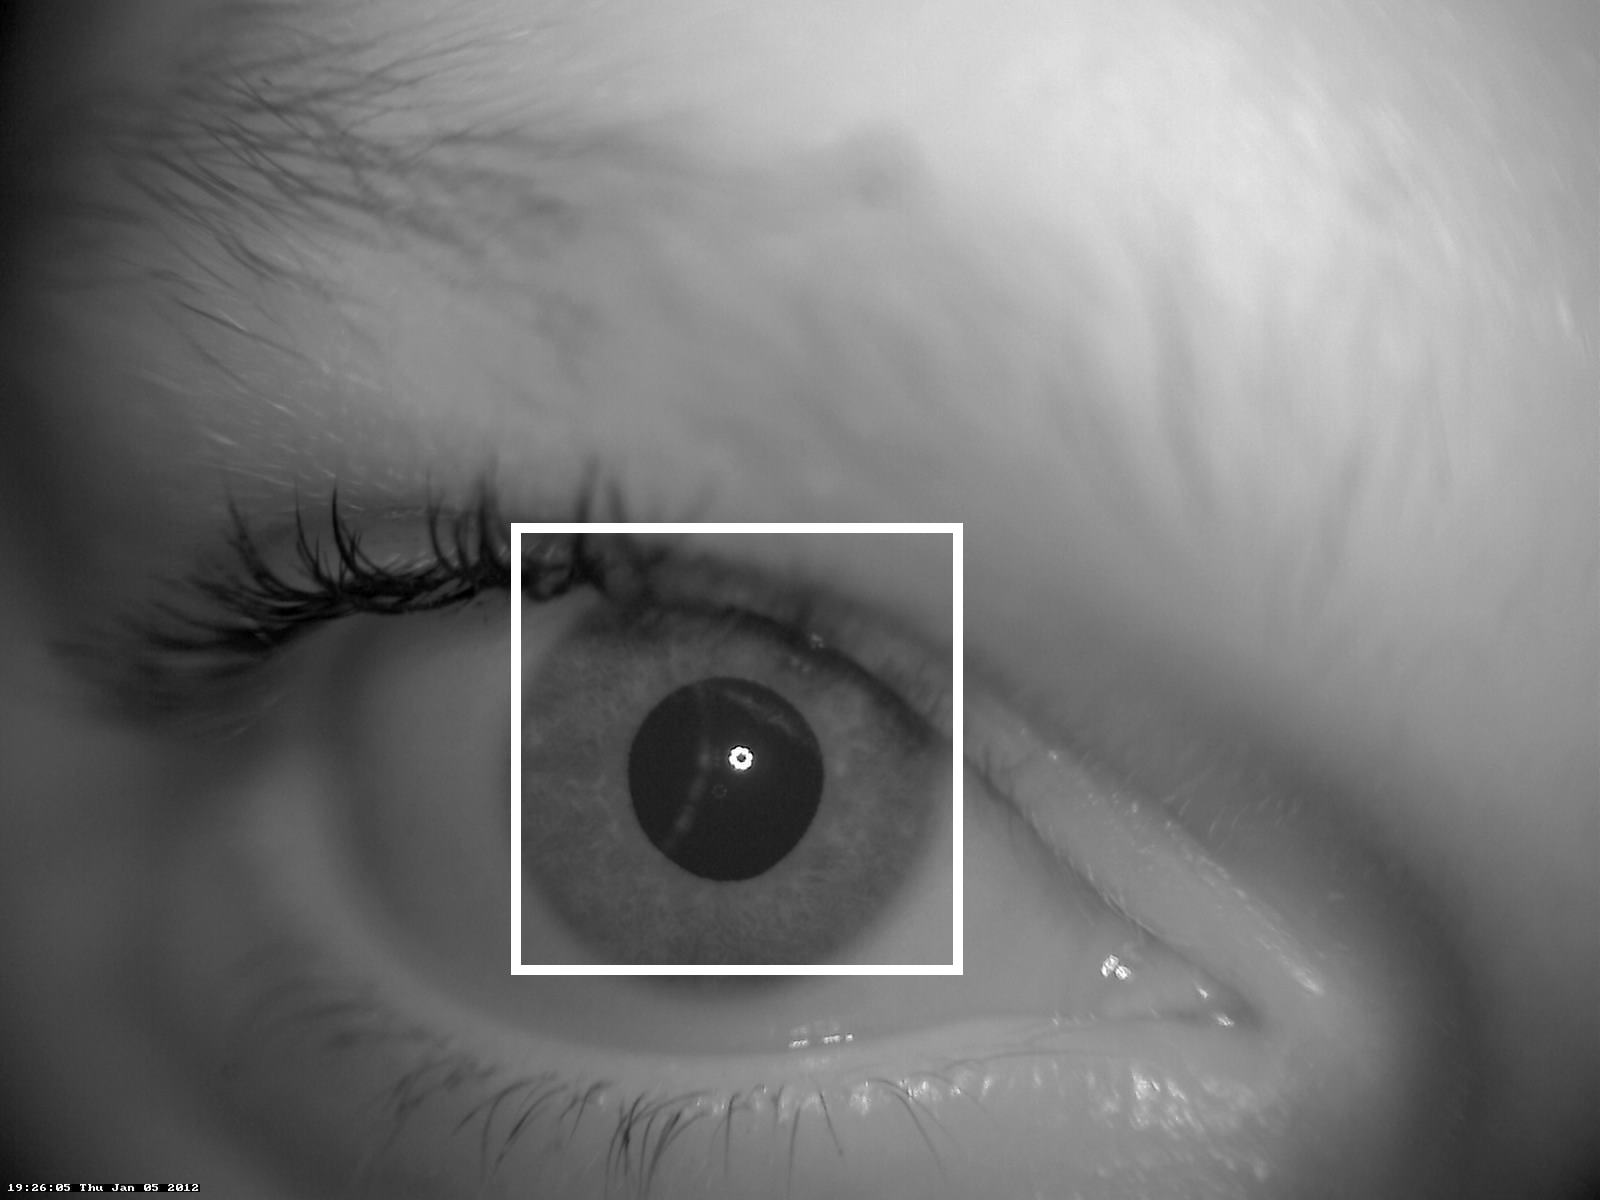
\includegraphics[scale=0.07]{obszar.jpg}
\end{center}
\end{figure}
\end{frame}

%---------------------------------------------------------------------------

\begin{frame}
\frametitle{Wykrycie źrenicy}
W wybranym fragmencie obrazu stosujemy operację binaryzacji w celu wyznaczenia źrenicy z dwoma progami: mniejsze od 60 oraz większe od 254 .
\begin{figure}
\begin{center}
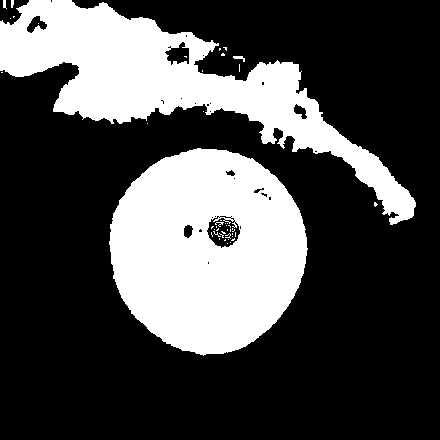
\includegraphics[scale=0.25]{bin.jpg}
\end{center}
\end{figure}
\end{frame}

%---------------------------------------------------------------------------

\begin{frame}
\frametitle{Wykrycie źrenicy}
Kolejno stosowane są operacje zamknięcia i dwukrotnego otwarcia (za drugim razem ze zwiększonym obiektem strukturalnym) w celu otrzymania koła określającego źrenicę.
\begin{columns}
	\column{0.3\textwidth}
		\begin{figure}
		\begin{center}
		
\includegraphics[scale=0.25]{zamkniecie.jpg}
		\end{center}
		\end{figure}
	\column{0.3\textwidth}
		\begin{figure}
		\begin{center}
		
\includegraphics[scale=0.25]{otwarcie1.jpg}
		\end{center}
		\end{figure}
	\column{0.3\textwidth}
		\begin{figure}
		\begin{center}
		
\includegraphics[scale=0.25]{otwarcie2.jpg}
		\end{center}
		\end{figure}
\end{columns}
\end{frame}

%---------------------------------------------------------------------------

\begin{frame}
\frametitle{Wykrycie źrenicy}
Ostatnim etapem jest zastosowanie algorytmu czyszczenie brzegu na wybranym obszarze. Pozostały obiekt jest źrenicą.
\begin{columns}
	\column{0.5\textwidth}
		\begin{figure}
		\begin{center}
		
\includegraphics[scale=0.25]{roi1.jpg}
%		\caption{Obraz przed czyszczeniem brzegów}
		\end{center}
		\end{figure}
	\column{0.5\textwidth}
		\begin{figure}
		\begin{center}
		
\includegraphics[scale=0.25]{roi2.jpg}
%		\caption{Obraz po czyszczenu brzegów}
		\end{center}
		\end{figure}
\end{columns}
\end{frame}

%---------------------------------------------------------------------------

\begin{frame}
\frametitle{Wykrycie tęczówki}
Sposób wykrywania tęczówki jest zgodny z patentem Daugmana; został zastosowany również w zeszłorocznej pracy. Po wykonaniu algorytmu widzimy obszar na zdjęciu, w którym znajduje się tęczówka.
\begin{figure}
\begin{center}
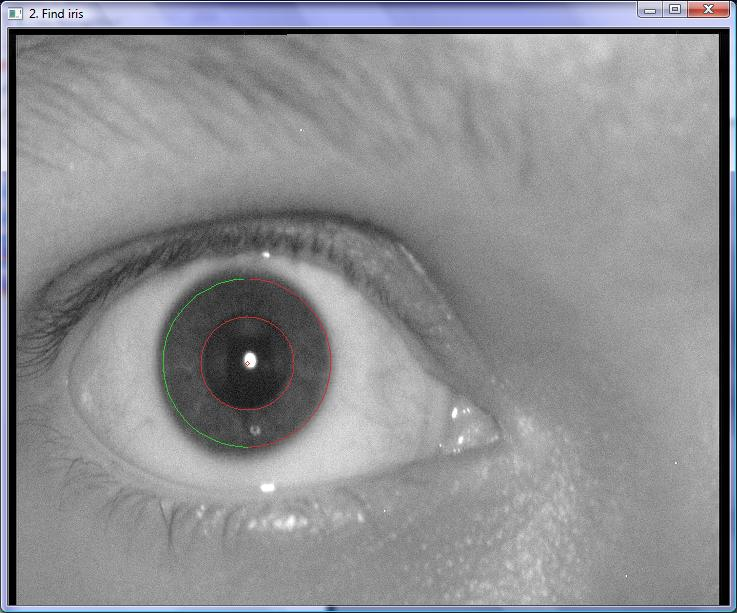
\includegraphics[scale=0.25]{teczowka_nasza.jpg}
\end{center}
\end{figure}
\end{frame}

%---------------------------------------------------------------------------

\begin{frame}
\frametitle{Tworzenie kodu tęczówki}
Kod tęczówki jest tworzony w następujący sposób:
\begin{itemize}
\item Wybierana jest odpowiednia liczba obszarów, tak, aby powstał kod o długości 2048 bitów,
\item Każdy z obszarów jest filtrowany filtrami Gabora (jest ich 8, każdy o innym kierunku),
\item Sumowane są otrzymane liczby zespolone,
\item Koduje się sumy, osobno część rzeczywistą oraz urojoną: 1 dla sumy danej części większej od 0, 0 dla sumy danej części mniejszej lub równej 0.
\end{itemize}
\end{frame}

%---------------------------------------------------------------------------

\begin{frame}
\frametitle{Porównywanie kodów}
Kody porównuje się licząc ile jest różnych pikseli dla dwóch kodów w stosunku do długości kodu. Używany jest wzór:
$$ H = \frac{\sum XOR(A,B)}{2048} $$
gdzie:
$A, B$ - porównywane kody tęczówek, każdy o długości 2048 bitów.\\

Uznaje się, że dwa zdjęcia są obrazami tej samej tęczówki w przypadku, gdy wyliczona odległość Hamminga ma wartość poniżej 0.18.
\end{frame}

%---------------------------------------------------------------------------
\begin{frame}
\frametitle{Baza danych programu}
W celu poszerzenia funkcjonalności aplikacji, postanowiono rozbudować istniejącą bazę danych systemu. Schemat przebudowanej bazy wygląda następująco:

\begin{figure}
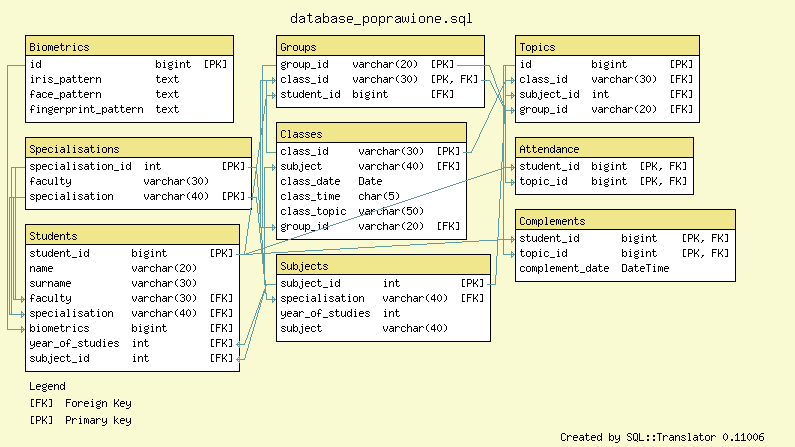
\includegraphics[scale=0.3]{diagram.png}
\end{figure}
\end{frame}

\begin{frame}
\frametitle{Wybrane tabele}

Wśród wielu tabel bazy, na szczególną uwagę zasługują relacje Biometryki (Biometrics), Zdjęcia (Photos), Obecność (Attendance) oraz Odrabiający (Complements).
\begin{figure}
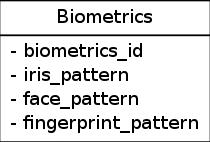
\includegraphics{biometrics.png}
\end{figure}
\end{frame}

\begin{frame}
\frametitle{Wybrane tabele}

\begin{figure}
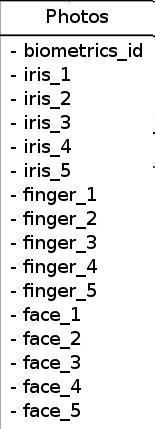
\includegraphics{photos.png}
\end{figure}
\end{frame}

\begin{frame}
\frametitle{Podstawowy interfejs aplikacji}
W podstawowej wersji programu obecny był jedynie uproszczony interfejs aplikacji.
\begin{figure}
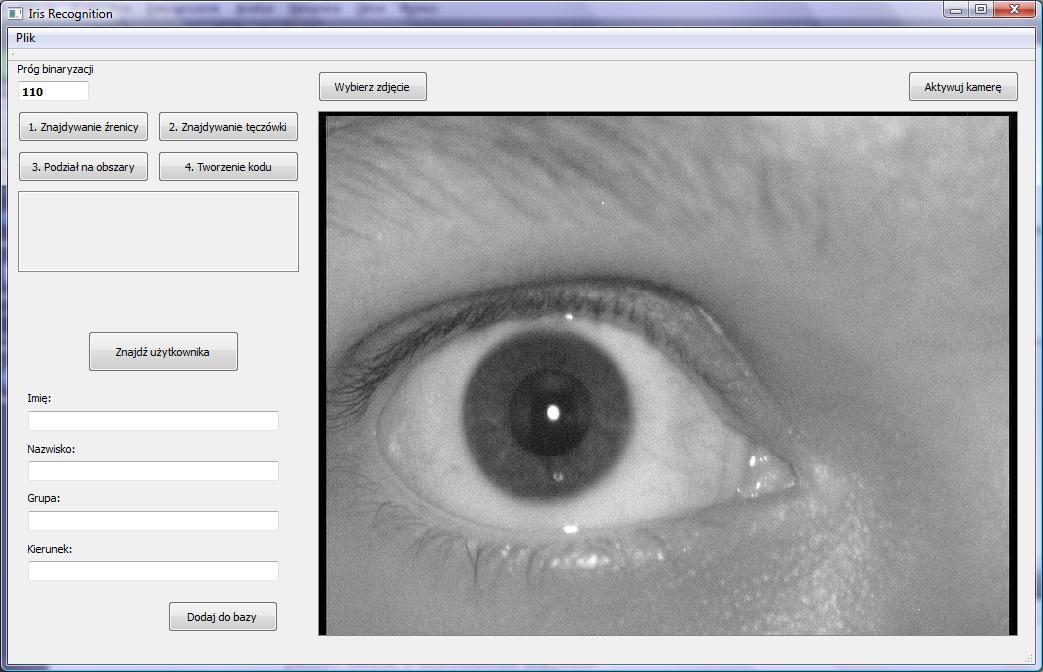
\includegraphics[scale=0.2]{oknoGlowne.jpg}
\end{figure}
\end{frame}

\begin{frame}
\frametitle{Rozszerzony interfejs aplikacji}
Rozbudowa bazy danych wiązała się z poszerzeniem interfejsu programu. Dodano zakładki umożliwiające zaawansowane korzystanie z funkcji oferowanych przez nową bazę. Zakładki dostępne są po naciśnięciu przycisku Zaawansowane opcje dodawania w głównym oknie aplikacji.

\end{frame}


\begin{itemize}
\item Zaawansowane opcje dodawania - zakładki: Dodaj kierunek, Dodaj przedmiot, Dodaj temat, Dodaj grupę, Dodaj zajęcia
\item Generowanie listy obecności
\end{itemize}
\end{frame}

\begin{frame}
\frametitle{Okno główne aplikacji}
Po przebudowie aplikacji, okno główne przyjęło postać:

\end{frame}

\begin{frame}
\frametitle{Zakładka Dodaj kierunek}
Pierwszą zakładką, w której możliwe jest uzupełnienie danych, jest Dodaj kierunek. Pozwala ona na dodanie specjalności o podanej nazwie i wydziale.

\end{frame}

\begin{frame}
\frametitle{Zakładka Dodaj przedmiot}
W zakładce drugiej możliwe jest dodanie przedmiotu o określonej nazwie, odbywającym się na konkretnym kierunku i roku studiów:

\end{frame}

\begin{frame}
\frametitle{Zakładka Dodaj temat}
W kolejnej zakładce można w ramach przedmiotu dodać realizowane tematy:

\end{frame}

\begin{frame}
\frametitle{Zakładka Dodaj grupę}
Zakładka Dodaj grupę pozwala na utworzenie grup studentów mających zajęcia w określone dni tygodnia i danych godzinach:

\end{frame}

\begin{frame}
\frametitle{Zakładka Dodaj zajęcia}
W zakładce Dodaj zajęcia możliwe jest dodanie zajęć z przedmiotu, wraz z podaniem terminu ich odbycia się oraz grupy i realizowanego tematu:

\end{frame}

\begin{frame}
\frametitle{Iplementacja}
\begin{itemize}
\item Język C++.
\item Biblioteka do przetwarzania obrazów: OpenCV.
\item Biblioteka do tworzenia interfejsu graficznego: Qt.
\item System zarządzania bazami danych: SQLite.
\end{itemize}
\end{frame}

%---------------------------------------------------------------------------

\begin{frame}
\frametitle{Wyniki testów}
\begin{table}
\begin{center}
\label{tab:druga1}
\begin{tabular}{|c|c|c|c|c|c|c|c|c|c|c|c|c|c|c|c|c|c|c|l|}
\hline

 & A1 & A2 & A3 & B1 & B2 & B3 & C1 & C2\\ \hline
A1  & \multicolumn{1}{>{\columncolor{green}}c|}{ 0} & \multicolumn{1}{>{\columncolor{green}}c|}{0,114} & \multicolumn{1}{>{\columncolor{green}}c|}{0,121} & \multicolumn{1}{>{\columncolor{red}}c|}{0,194} & \multicolumn{1}{>{\columncolor{red}}c|}{0,196} & \multicolumn{1}{>{\columncolor{red}}c|}{0,195} & \multicolumn{1}{>{\columncolor{red}}c|}{0,212} & \multicolumn{1}{>{\columncolor{red}}c|}{0,213}\\ \hline
A2  & \multicolumn{1}{>{\columncolor{green}}c|}{ 0,114} & \multicolumn{1}{>{\columncolor{green}}c|}{0} & \multicolumn{1}{>{\columncolor{green}}c|}{0,078} & \multicolumn{1}{>{\columncolor{red}}c|}{0,192} & \multicolumn{1}{>{\columncolor{red}}c|}{0,186} & \multicolumn{1}{>{\columncolor{red}}c|}{0,184} & \multicolumn{1}{>{\columncolor{red}}c|}{0,207} & \multicolumn{1}{>{\columncolor{red}}c|}{0,21}\\ \hline
A3  & \multicolumn{1}{>{\columncolor{green}}c|}{ 0,121} & \multicolumn{1}{>{\columncolor{green}}c|}{0,078} & \multicolumn{1}{>{\columncolor{green}}c|}{0} & \multicolumn{1}{>{\columncolor{red}}c|}{0,198} & \multicolumn{1}{>{\columncolor{red}}c|}{0,194} & \multicolumn{1}{>{\columncolor{red}}c|}{0,189} & \multicolumn{1}{>{\columncolor{red}}c|}{0,207} & \multicolumn{1}{>{\columncolor{red}}c|}{0,213}\\ \hline
B1  & \multicolumn{1}{>{\columncolor{red}}c|}{ 0,194} & \multicolumn{1}{>{\columncolor{red}}c|}{0,192} & \multicolumn{1}{>{\columncolor{red}}c|}{0,198} & \multicolumn{1}{>{\columncolor{green}}c|}{0} & \multicolumn{1}{>{\columncolor{green}}c|}{0,124} & \multicolumn{1}{>{\columncolor{green}}c|}{0,108} & \multicolumn{1}{>{\columncolor{red}}c|}{0,2} & \multicolumn{1}{>{\columncolor{red}}c|}{0,206}\\ \hline
B2  & \multicolumn{1}{>{\columncolor{red}}c|}{ 0,196} & \multicolumn{1}{>{\columncolor{red}}c|}{0,186} & \multicolumn{1}{>{\columncolor{red}}c|}{0,194} & \multicolumn{1}{>{\columncolor{green}}c|}{0,124} & \multicolumn{1}{>{\columncolor{green}}c|}{0} & \multicolumn{1}{>{\columncolor{green}}c|}{0,065} & \multicolumn{1}{>{\columncolor{red}}c|}{0,191} & \multicolumn{1}{>{\columncolor{red}}c|}{0,203}\\ \hline
B3  & \multicolumn{1}{>{\columncolor{red}}c|}{ 0,195} & \multicolumn{1}{>{\columncolor{red}}c|}{0,184} & \multicolumn{1}{>{\columncolor{red}}c|}{0,189} & \multicolumn{1}{>{\columncolor{green}}c|}{0,108} & \multicolumn{1}{>{\columncolor{green}}c|}{0,065} & \multicolumn{1}{>{\columncolor{green}}c|}{0} & \multicolumn{1}{>{\columncolor{red}}c|}{0,199} & \multicolumn{1}{>{\columncolor{red}}c|}{0,202}\\ \hline
C1  & \multicolumn{1}{>{\columncolor{red}}c|}{ 0,212} & \multicolumn{1}{>{\columncolor{red}}c|}{0,207} & \multicolumn{1}{>{\columncolor{red}}c|}{0,207} & \multicolumn{1}{>{\columncolor{red}}c|}{0,2} & \multicolumn{1}{>{\columncolor{red}}c|}{0,191} & \multicolumn{1}{>{\columncolor{red}}c|}{0,199} & \multicolumn{1}{>{\columncolor{green}}c|}{0} & \multicolumn{1}{>{\columncolor{green}}c|}{0,121}\\ \hline
C2  & \multicolumn{1}{>{\columncolor{red}}c|}{ 0,213} & \multicolumn{1}{>{\columncolor{red}}c|}{0,21} & \multicolumn{1}{>{\columncolor{red}}c|}{0,213} & \multicolumn{1}{>{\columncolor{red}}c|}{0,206} & \multicolumn{1}{>{\columncolor{red}}c|}{0,203} & \multicolumn{1}{>{\columncolor{red}}c|}{0,202} & \multicolumn{1}{>{\columncolor{green}}c|}{0,121} & \multicolumn{1}{>{\columncolor{green}}c|}{0}\\ \hline
C3  & \multicolumn{1}{>{\columncolor{red}}c|}{ 0,208} & \multicolumn{1}{>{\columncolor{red}}c|}{0,207} & \multicolumn{1}{>{\columncolor{red}}c|}{0,208} & \multicolumn{1}{>{\columncolor{red}}c|}{0,198} & \multicolumn{1}{>{\columncolor{red}}c|}{0,202} & \multicolumn{1}{>{\columncolor{red}}c|}{0,204} & \multicolumn{1}{>{\columncolor{green}}c|}{0,145} & \multicolumn{1}{>{\columncolor{green}}c|}{0,093}\\ \hline
D1  & \multicolumn{1}{>{\columncolor{red}}c|}{ 0,186} & \multicolumn{1}{>{\columncolor{red}}c|}{0,197} & \multicolumn{1}{>{\columncolor{red}}c|}{0,201} & \multicolumn{1}{>{\columncolor{red}}c|}{0,219} & \multicolumn{1}{>{\columncolor{red}}c|}{0,216} & \multicolumn{1}{>{\columncolor{red}}c|}{0,213} & \multicolumn{1}{>{\columncolor{red}}c|}{0,21} & \multicolumn{1}{>{\columncolor{red}}c|}{0,211}\\ \hline
D2  & \multicolumn{1}{>{\columncolor{red}}c|}{ 0,186} & \multicolumn{1}{>{\columncolor{red}}c|}{0,194} & \multicolumn{1}{>{\columncolor{red}}c|}{0,197} & \multicolumn{1}{>{\columncolor{red}}c|}{0,212} & \multicolumn{1}{>{\columncolor{red}}c|}{0,208} & \multicolumn{1}{>{\columncolor{red}}c|}{0,208} & \multicolumn{1}{>{\columncolor{red}}c|}{0,211} & \multicolumn{1}{>{\columncolor{red}}c|}{0,214}\\ \hline
D3  & \multicolumn{1}{>{\columncolor{red}}c|}{ 0,185} & \multicolumn{1}{>{\columncolor{red}}c|}{0,199} & \multicolumn{1}{>{\columncolor{red}}c|}{0,197} & \multicolumn{1}{>{\columncolor{red}}c|}{0,223} & \multicolumn{1}{>{\columncolor{red}}c|}{0,216} & \multicolumn{1}{>{\columncolor{red}}c|}{0,211} & \multicolumn{1}{>{\columncolor{red}}c|}{0,216} & \multicolumn{1}{>{\columncolor{red}}c|}{0,222}\\ \hline
\end{tabular}
\end{center}
\end{table}
\end{frame}

%---------------------------------------------------------------------------

\begin{frame}
\frametitle{Wnioski}
\begin{itemize}
\item Udało się skonstruować system do identyfikacji na podstawie tęczówki.
\item Najważniejsze jest uzyskanie dobrego obrazu, z jak najmniejszą liczbą zakłóceń.
\item Stworzone stanowisko nie jest przenośne.
\item Tęczówka na zdjęciu musi być duża, potrzeba jest dużej liczby szczegółów tęczówki.
\item Najtrudniejszym etapem podczas tworzenia kodu tęczowki jest segmentacja źrenicy.
\end{itemize}
\end{frame}

\begin{frame}
\frametitle{Koniec}

\begin{block}{}
Dziękujemy za uwagę.\\
Pytania?

\end{block}

\end{frame}

%---------------------------------------------------------------------------


\end{document}

